{\let\clearpage\relax
\chapter{Arbeitsplanung}}
\label{sec:ablaufplanung}

\section{Vorgangsliste und Abhängigkeiten}
Zur Ablaufplanung wird eine \textbf{Vorgangsliste} mit 12 Arbeitspaketen erstellt. Diese diente als Grundlage für:
\begin{itemize}
  \item Identifikation von Abhängigkeiten,
  \item Schätzung von Dauern und Zeitpunkten,
  \item Zuordnung von Ressourcen.
\end{itemize}

Die Abhängigkeiten zwischen Arbeitspaketen werden durch Einschätzung und Erfahrung identifiziert. Es ergeben sich sowohl \textbf{stringente} als auch \textbf{parallele Abläufe.}

Die Aufwandsschätzung erfolgte mithilfe der \textbf{gewichteten Drei-Punkt-Schätzung}:
\[
A = \frac{A_o + 2 \cdot A_w + A_p}{4}
\]
Dabei stehen $A_o$, $A_w$ und $A_p$ für den optimistischen, wahrscheinlichsten und pessimistischen Aufwand.

\begin{figure}[ht]
	\centering
	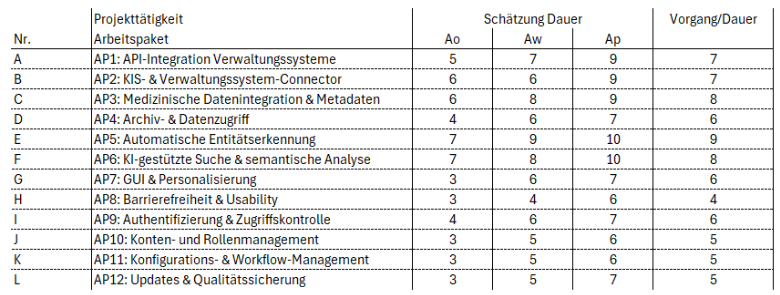
\includegraphics[width=0.9\textwidth]{fig/vorrangliste.png}
	\caption{Vorrangliste}
	\label{fig:vorrangliste}
\end{figure}

\section{Netzpläne und Zeitberechnungen}
Basierend auf der Vorgangsliste werden \textbf{Netzpläne} erstellt, um zeitliche Abläufe zu berechnen. Dabei kamen zwei Verfahren zum Einsatz:

\subsection{Vorwärtsrechnung}
\begin{itemize}
  \item Frühester Anfang ($FA$) beginnt bei 0 bei Startpaketen.
  \item Frühestes Ende: $FE = FA + \text{Dauer}$.
  \item Für Folgepakete: $FA = \max(FE_{\text{Vorgänger}})$.
\end{itemize}

\subsection{Rückwärtsrechnung}
\begin{itemize}
  \item Spätestes Ende ($SE$) des Endpakets entspricht dem $FE$.
  \item Spätester Anfang: $SA = SE - \text{Dauer}$.
  \item Für Vorgänger: $SE = \min(SA_{\text{Nachfolger}})$.
\end{itemize}

\begin{figure}[ht]
	\centering
	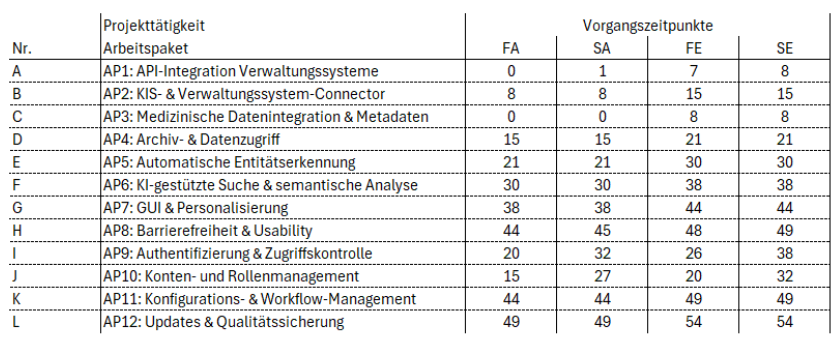
\includegraphics[width=0.9\textwidth]{fig/vorrangliste2.png}
	\caption{Vorrangzeitpunkte}
	\label{fig:vorrangzeitpunkte}
\end{figure}

\subsection{Pufferzeiten}
Pufferzeit beschreibt den Zeitrahmen, in dem ein Arbeitspaket ohne Projektverzögerung verschoben werden kann:
\[
Puffer = SE - FE = SA - FA
\]

\textbf{Beispiel:} Für AP10 ergibt sich ein Puffer von $32 - 20 = 27 - 15 = 12$.

\subsection{Kritische Aktivitäten}
Im Netzplan werden \textbf{kritische Pfade} identifiziert. Diese Arbeitspakete besitzen keinen Puffer und dürfen nicht verzögert werden, da sie direkt das Projektende beeinflussen. Der \textbf{kritische Pfad} wird rot markiert.

\subsection{Umrechnung in Wochendauer}
\begin{itemize}
	\item Gesamtprojektdauer: $3 \; Jahre = 36 \; Monate = 156 \; Wochen$
	\item Gesamtaufwand des kritischen Pfads: 57 Einheiten (inkl. AP13 - Dokumentation \& Schulung)
	\item Dauer des kritischen Pfads = 57 2,74 = 156,18 Wochen
\end{itemize}
\[
	\frac{156 \; Wochen}{57 \; Aufwand} \approx 2,74 \frac{Wochen}{Aufwand}
\]
\begin{figure}[ht]
	\centering
	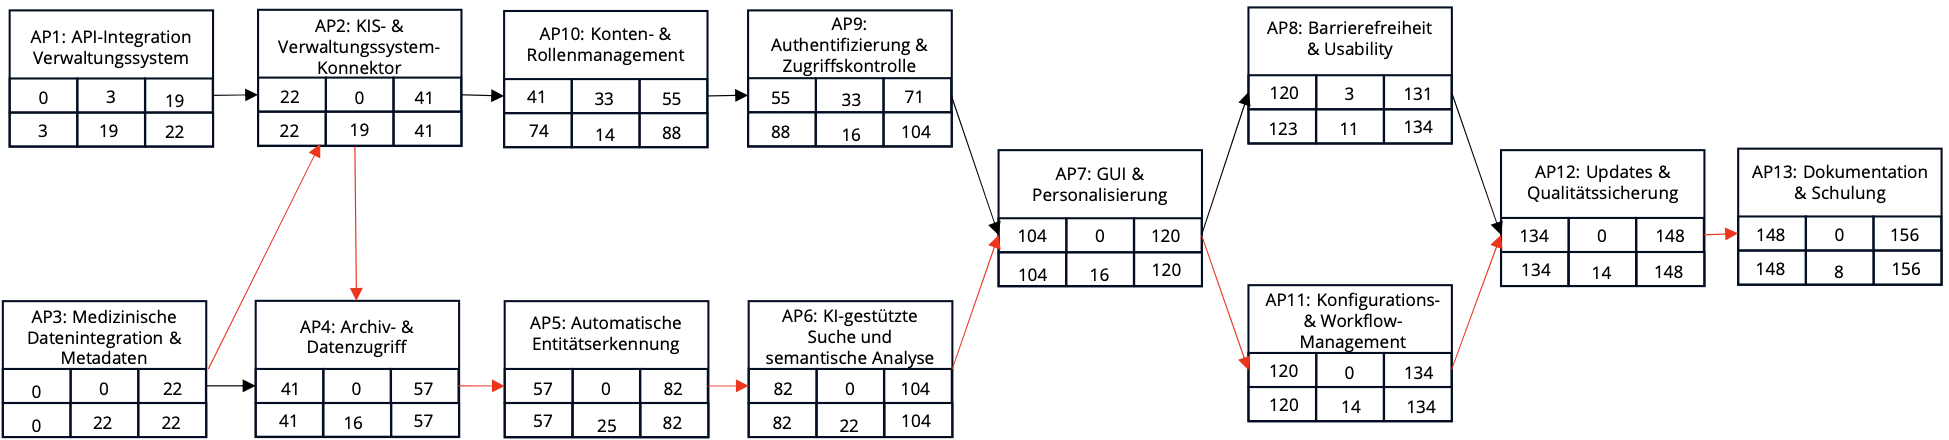
\includegraphics[width=1\textwidth]{fig/Netzplan.png}
	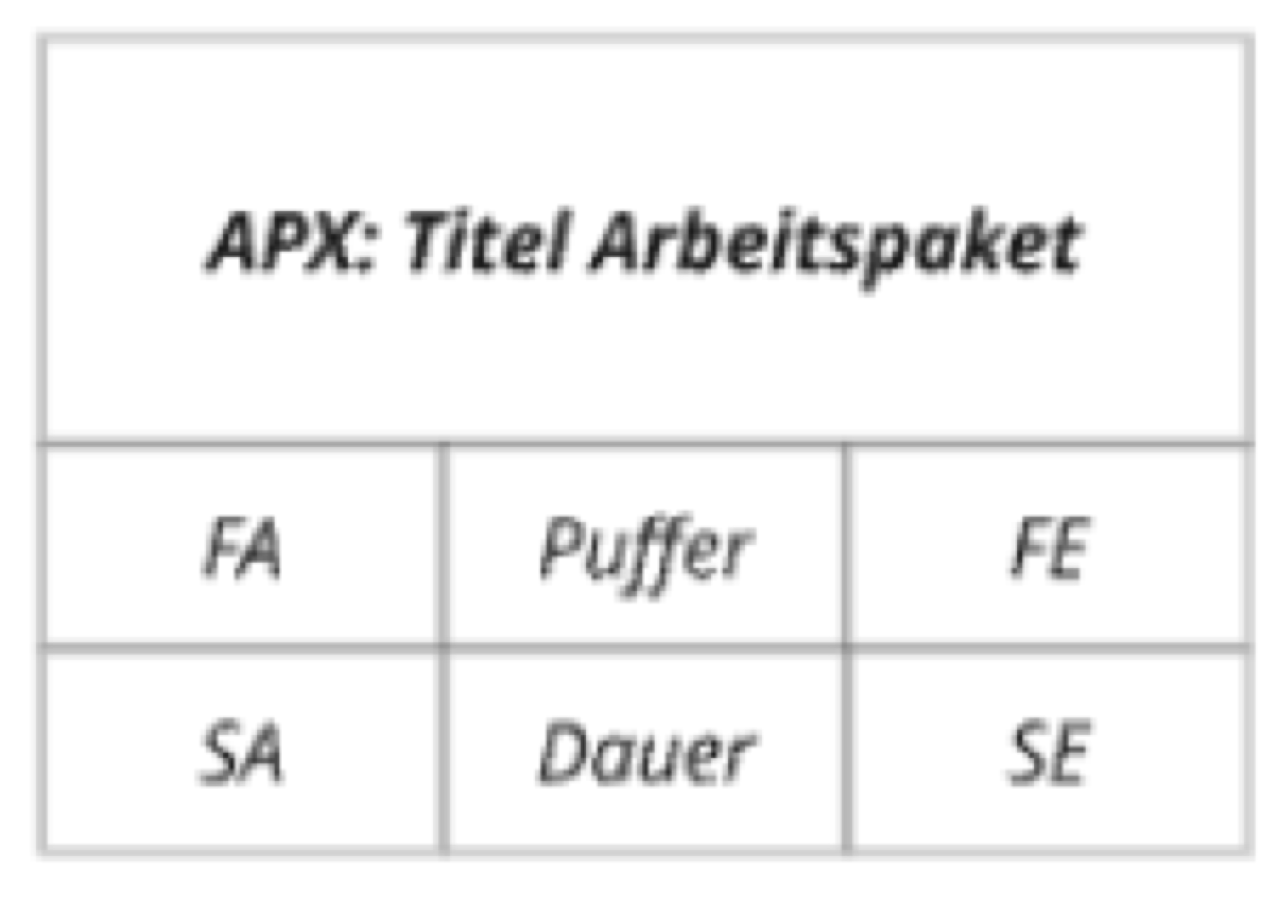
\includegraphics[width=0.15\textwidth]{fig/Netzplan info.png}
	\caption{Netzplan mit Markiertem Kritischen Pfad}
	\label{fig:netzplan}
\end{figure}
\pagebreak
%\section{Ressourcenzuordnung}
%Ressourcen werden zwei Hauptkategorien zugeordnet:

%\begin{itemize}
%  \item \textbf{Personalgruppen} - MA (z.B. Backend, DevOps, UX, QA)
%  \item \textbf{Sachmittel} - SM (z.B. Rechentechnik, Werkzeuge, Methoden)
%\end{itemize}
%Jedes Arbeitspaket hat einen gewissen bedarf an unterschiedlichen Gruppen und dieser wird ihnen zugeordnet.
%\\
%Eine detaillierte Zuordnung der Sachmittel erfolgte auf Ebene einzelner Arbeitspakete. Beispiele:
%\begin{itemize}
%  \item \textbf{AP1} – API-Gateway, Postman, CI-Tools
%  \item \textbf{AP5} – GPU-Server, NLP-Toolkits, Annotierungssoftware
%  \item \textbf{AP9} – IAM-Systeme, VPN, Sicherheits-Scanner
%\end{itemize}
